\documentclass[spanish,12pt,letterpapper]{article}
\usepackage{babel}
\usepackage[utf8]{inputenc}
\usepackage{graphicx}
\begin{document}
	\begin{titlepage}
		\begin{center}
			
\includegraphics[width=0.6\textwidth]{./logoUnADM}~\\[1cm] 
			\textsc{Universidad Abierta y a Distancia de México}\\[0.8cm]
			\textsc{Desarrollo de Software}\\[1.8cm]
			
			\textbf{ \Large Actividad 2. Los DBMS y el diseño de base de datos}\\[3cm]
			
			Diego Antonio Plascencia Lara\\ ES1421004131 \\[0.4cm]
			Facilitador(a): CESAR ALEXIE CHAN PUC  \\
			Materia: Diseño de Bases de Datos\\
			Grupo: DS-DDBD-1601-B1-003 \\
			Unidad: I \\
			
			\vfill México D.F\\{\today}
			
		\end{center}
	\end{titlepage}
	
	\section{Concepto de DBMS.\\}
	Un ``Database Management System'' es un conjunto de programas que permiten a los usuarios crear y mantener una base de datos de acuerdo a el ``ANSI/SPARC DBMS Report (1977)'', y este debe estar compuesto por capas que permiten manipular los datos, estas capas van desde la mas baja (el almacenamiento físico, el manejo de archivos o ``File System'').
	
	\section{Principales funciones de un DBMS}
	\begin{itemize}
	\item Permiten la concurrencia.
	\item Seguridad de control.
	\item Mantienen la integridad de los datos.
	\item Proveen de una copia de seguridad y recuperación.
	\item Redundancia de control.
	\item Permiten la independencia de datos.
	\item Provee un lenguaje de consulta no procedimental.
	\item Realiza una optimización de consultas automático
	\end{itemize}
	
	\pagebreak
	
	\section{Tipos de Usuarios en el DBMS}
	\begin{itemize}
	\item \textbf{Administrador.} Autoriza el acceso a la base de datos, coordina y monitorea su uso, así como adquiere los recursos de hardware y software.
	\item \textbf{Diseñadores.} Identifican los datos que deben ser almacenados y seleccionan las estructuras apropiadas que representan y almacenan estos datos.
	\item \textbf{Usuarios Finales. }Son las personas que para realizar su trabajo requieren del acceso a la base de datos.
	\item \textbf{Analista de sistemas.} Determina los requerimientos de los usuarios finales. 
	\item \textbf{Programadores.} Implementan las especificaciones del analista como programas.
	\end{itemize}
	
	\section{Aspectos}
	\subsection{Seguridad}	
	\begin{itemize}
	\item Ofrece protección a nivel archivo, todos los archivos almacenados en la BD son protegidos de su lectura por otras cuentas que no sean el superusuario.
	\item Esta configurada por defecto solo se permite la conexión de manera local y no por TCP/IP.
	\item Las conexiones pueden ser restringidas a una dirección IP.
	\item Hace uso de autenticaciones (usuario y contraseña) asi como de grupos y privilegios.
	\end{itemize}
	
	\subsection{Gestión}
	Se puede gestionar postgreSQL mediante la herramienta de cli por defecto que acepta cualquier operación SQL, asi como también existen interfaces gráficas, dos de ellas son ``PgAccess'' que viene incluida en la distribución de PostgreSQL y ``PgAdmin'' que es open source y uno de los mas populares. 
	
	\subsection{Transacción}
	Las transacciones son un conjunto de operaciones o instrucciones para la BD en las que se ejecutan todas y en caso de haber un error en el transcurso de estas se deshacen las instrucciones si realizadas hasta volver a un punto de integridad, es conocido como operación "todo o nada" y  en PostgreSQL se define con la sentencia ``BEGIN; ... COMMIT;'', por ejemplo:\\
	
	``BEGIN;\\
UPDATE accounts SET balance = balance - 100.00
    WHERE name = 'Alice';\\
-- etc etc\\
COMMIT;'' \\
	   
	\subsection{Definición de Datos}
	   \begin{itemize}
	   \item bool (true or false).
	   \item box (caja rectangular en 2D plano) / lseg (segmento de linea en 2D plano) / polygon / circle / line / path / point.
	   \item char (cadena de caracteres) / varchar (cadena variable).
	   \item cidr (ip v4 o dirección host). / inet
	   \item decimal.
	   \item float4 / float8.
	   \item int2 / int4 / int8.
	   \item interval.
	   \item money (moneda en formato us).
	   \item numeric
	   \item serial (id unico para indexacion y referencia cruzada)
	   \item date (día del calendario) / time / timetz (tiempo y zona horaria) / timestamp (fecha y hora)   
	   \end{itemize}
	   
	   \subsection{Arquitectura}
	   PostgreSQL tiene una arquitectura basica de ``Proceso por usuario cliente-servidor'' y consta de un proceso demonio supervisor (postmaster), la aplicación que interactúa con el usuario, y uno o mas servidores de bases de datos (el proceso mismo de postgres).\\
	   
	   Un solo proceso Postmaster gestiona una colección dada de bases de datos en un solo host. En la aplicación del usuario la libreria libpq realiza la llamada sobre la red a Postmaster y este inicia un nuevo proceso postgres.\\
	   
	   \begin{center}
	   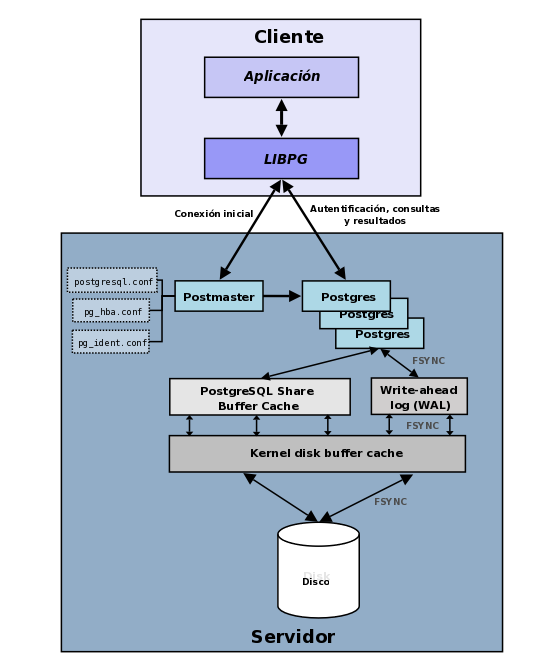
\includegraphics[width=0.8\textwidth]{./arqpq}~\\[1cm]
	   \end{center}
	   \pagebreak
	   

	
	\section{Instalación de el DBMS}
	Para este ejercicio seleccione PostgresSQL. Lo elegí por su licencia, que es un DBMS libre, de código abierto con licencia tipo MIT, sobre MySQL pues esta tiene licencia GPL y cuenta con licencias comerciales (requieren remuneración a Oracle); por su flexibilidad, no solo en cuanto a el código (cuenta con una librería en c), sino también por la flexibilidad en cuanto a la implementación pues permite trabajar como si fuera un RDBMS o NoSQL, e incluso un hibrido.\\
	
	\paragraph{Instalación mediante Repositorio\\}
	En mi caso realizare la instalación de postgres por medio de advanced packaging tool (apt) en GNU/Linux con el comando:\\
	`` \# apt-get install postgresql postgresql-contrib'' \\ 
	Y eso es todo, ahora podemos acceder a nuestro DBMS cambiándonos al usuario tipo root por defecto (postgres), con:\\
	 `` \# -i -u postgres ''\\
	 Y después iniciamos el programa con: `` \$ psql ''.\\
	 	 
	 \begin{center}
	 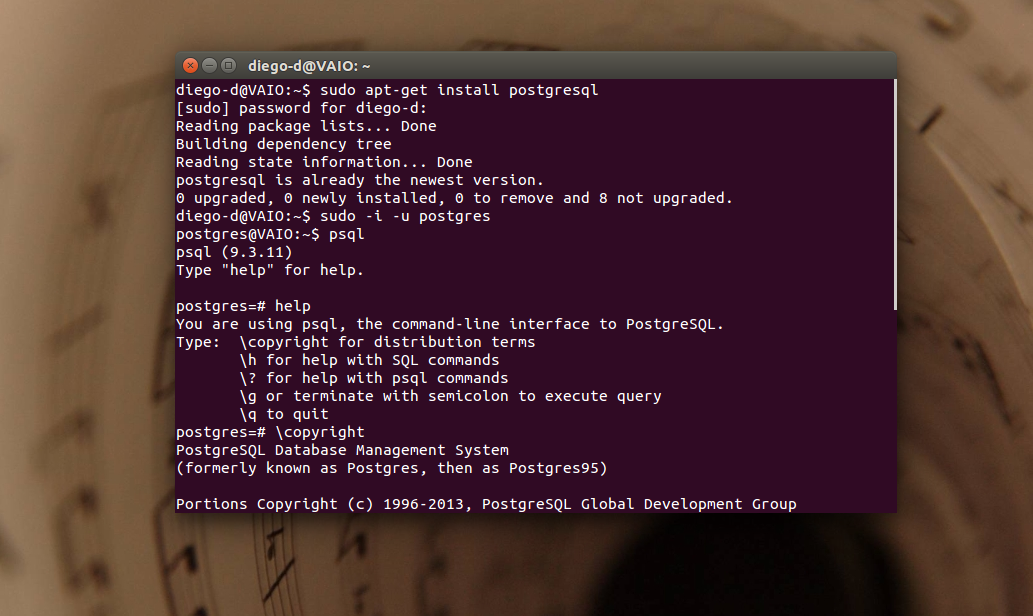
\includegraphics[width=1\textwidth]{./install_screenshot}~\\[1cm]
	 \end{center}
	 \pagebreak
	
	\section{Conclusión}
	Un DBMS es esencial en el diseño de las bases de datos, ya que en la practica es con lo que se interactuá para implementar el diseño y se debe conocer el DBMS para poder hacer el diseño mas optimo acorde al DBMS elegido, pues aunque es común entre los DBMS de bases de datos relacionales el lenguaje de de Consultas Estructurado para comunicarse a través del DML, pueden variar ciertas instrucciones o implementaciones, puesto que incluso podemos encontrarnos casos como tener que implementar un diseño híbrido (relacional y no-relacional).
	 
	
	\pagebreak
	\begin{thebibliography}{9}
		\bibitem{rrhopkins} Robert J. Robbins. 
		\emph{Database Fundamentals}. Johns Hopkins University, [Disponible en: http://www.esp.org/db-fund.pdf].
		
		\bibitem{elmasriynavathe} Ramez Elmasri and Shamkant Navathe. 
		\emph{Fundamentals of Database Systems}. Pearson Education, [Disponible en: http://tinman.cs.gsu.edu/~raj/4710/f11/Ch01.pdf].
		
		\bibitem{psqldocs} The PostgreSQL Development Team. 
		\emph{PostgreSQL 7.0 Docs}. PostgreSQL, [Disponible en: http://www.postgresql.org/docs/7.0/static/postgres.htm].
		

	\end{thebibliography}

\end{document}